\chapter{Neuro-Fuzzy-Modelle: Implementierung des ANFIS-Ansatzes}

In der folgenden Kapitel stelle ich die Aufsetzung des ANFIS-Ansatzes in Python vor. Während der Ausarbeitungszeit habe ich mich mit der Bibliothek für Neuronale Netze Tensorflow gesetzt. Tensorflow ist ein Produkt von Google und eine API für Erstellung von Neuronalen Netzen. Eine weitere Funktionalität, die die Bibliothek anbietet, ist die einfache Migration von erstellten Neuronalen Netzen. Tensorflow bietet die Möglichkeit, einfach Modelle nach den unterstützten Programmiersprachen zu exportieren, in disem Sinne auch nach C++.

In diesem Kapitel wird so vorgegangen, dass zu jedem Programmcode eine Erklärung gegeben wird. Der vorrige Kapitel geht auf die eigentliche Struktur und theoretische Aufsetzung eines ANFIS-Models in einem Neuronalen Netz. Laut dem Kapitel \ref{ANFIS} besteht ein ANFIS-System aus sechs Schichten (zwei äußere und vier inneren Schichten). Über die erste Schicht erfolgt die Eingabe im Netz. Die weiteren fünf Schichten führen einfache mathematische Funktionen aus.

\section{ANFIS-Klasse}\label{anfis-klasse}

Das Neuro-Fuzzy-Model wird nach dem bekannten ANFIS-Model eingerichtet. Das Model hat insgesammt 6 Schichten, 2 Außen- und 4 Innenschichten. Das ANFIS-Model wird in einer Klassendatei ausgelagert. Die Klasse verfügt über mehrere Methoden, einige davon Hilfsmethoden. Folglich werden die Wichtigsten davon in Unterkapiteln gestellt.
\subsection{Konstruktor}\label{konstruktor}

Die ANFIS-Klasse vefügt über einen einzigen Konstruktor. 

\begin{lstlisting}[language=Python]
# gradient_type defines the batch size to be used for learning
# 0-type = Stochastic Gradient Descent
# 1-type = Mini-Batch Gradient Descent, 30 samples from the training data
# 2-type = Batch Gradient Descent
def __init__(self, num_sets, path=None, gradient_type=0, mf_type=0):
...
\end{lstlisting}

Er hat einen Pflicht- und drei Optionalparameter - \emph{num\_sets} und entsprechend \emph{path}, \emph{mf\_type}, \emph{gradient\_type}. Der Parameter \emph{num\_sets} besagt wie viele Fuzzy-Mengen pro Eingangsgröße zu erstellen sind. Der Pfad wird durch ein String - \emph{path} - gegeben. Weiterhin unterscheide ich zwischen zwei Weisen der Berechnung von Zugehörigkeit. Anschliesend ergibt die Variable \emph{gradient\_type} die Größe der Trainingsdaten, oder die Art des Gradient-Descents. Es unterscheiden sich drei Arten von Gradient Descent Verfahren -
Stochastic, Mini-Batch und Batch Gradient Descent Verfahren. Die gegebene Anordnung der Begriffe entspricht der in dem Programmcode, sprich \emph{gradient\_type=0} entspricht dem stochastischen Verfahren. Der Wert \emph{1} heißt, dass das Mini-Batch ausgewählt wird und \emph{2} - Batch Gradient Descent. Die drei Arten unterscheiden sich in dem Punkt, dass die Variablen zu Unterschiedlichen Zeitpunkten angepasst werden. Bei dem stochastischen Verfahren werden die Parameter nach jeder Bearbeitung von Trainingspaaren verändert. Bei dem Mini-Batch wird jeweils nach der Bearbeitung von gewisser Anzahl an Datenelementen. Eine übliche Anzahl ist meistens zwischen 30 und 500 Trainingsdaten pro Iteration, jedoch ist das weniger als der Gesamtmenge. Der Batch Gradient Verfahren nimmt die ganze Datenmenge und führt mit denen einen Lernzug. Die Erkenntnisse aus den Tests werde ich in dem nächsten Kapitel beschreiben.

Der Konstruktor umfasst Definition der benötigten Variablen und die Erstellung des Models. Zu beginn werden die Trainingsdaten aus einer Datei gelesen. Durch die Struktur des Datensatzes wird die Anzahl der Eingangvariablen in dem Netz bestimmt. Die Datenpaar sind zeileinweise aufgebaut. In der Zeile werden zu bestimten Eingaben die Soll-Ergebnisse gegeben. Die letzte Spalte liefert die Sollwerte und in den Spalten davor werden die Eingangswerte geschrieben, sodass zum Beispiel in der ersten Spalte \(\mathbf{x_1}\), in der zweiten \(\mathbf{x_2}\) usw. und in der letzen der Erwartungswert steht. Üblicherweise arbeite ich mit einer Eingangsgröße, somit hat eine Datei zwei Spalten. 
Falls das gegebene Pfad gültig ist, werden vier Felder erstellt, zwei jeweils fürs Lernen und die Prüfung. Falls der Parameter \(\textit{fulltrain}\) auf \(\textit{wahr}\) gesetzt ist, werden die Daten nicht aufgeteilt. Bei dem Vorderen werden die Daten so getrennt, dass drei viertel der Datensätze fürs Training und ein viertel der Daten für die Bewertung des gelernten Modells verwendet werden. 
Anschließend wird mit der Konstruktion des Neuronalen Netzes fortgefahren. Folglich werden sechs weiteren Hilfsmethoden ausgeführt, die die Schichten des Neuronalen Netzes ausbauen. Diese werde ich etwas ausführlicher vorstellen.

Ein Beispiel für einen Aufruf des Konstruktors:

\begin{lstlisting}[language=Python]
#...
# the default mf_type and gradient_type 
# are set to 0, although gradient_type 0 is not the most optimal
f = Anfis(num_sets=num_sets, 
	path="../utils/sinus.out", gradient_type=0, mf_type=0)
\end{lstlisting}

\subsection{Eingangsschicht (FirstLayer)}\label{eingangsschicht-first-layer}

Die Definition der Eingangsschicht erfolgt in der Funktion \emph{first\_layer()}. Die Methode erhält keine Parameter und initialisiert zwei Tensoren für die Eingangsgrößen \textbf{X} und \textbf{Y}. In Tensorflow können Eingaben an mehreren Stellen im Netzt eingeführt werden, was hier auch der Fall für die \textbf{Y-Variable} ist. Die \textbf{Y-Variable} wird in der Fehlerfunktion gebraucht und sie enthält alle Soll-Ergebnisse.


\begin{lstlisting}[language=Python]
#...
# three different types for gradient descent type
# so we have three types of batch size, 
# wich defines the amount of elements to be evaluated in one iteration
if self.gradient_type == 0:
	self.batch_size = self.num_inputs
elif self.gradient_type == 1:
	self.batch_size = int((1 / 5) * (len(self.train_x_arr)))  
elif self.gradient_type == 2:
	self.batch_size = len(self.train_x_arr)
# input variable
self.x = tf.placeholder(name="x", shape=(self.num_inputs, self.batch_size), 
	dtype=tf.float64)
# variable for expected result
# we define dtype=tf.float64, because of the size of the values
# that the model returns
self.y = tf.placeholder(name="y", shape=(self.batch_size), dtype=tf.float64)
#...
\end{lstlisting}

Die $\textbf{Variable X}$ ist ein Array, das eine Matrix mit $\textit{n (num\_inputs)}$ Zeilen (Werten) und $\textit{batch\_size}$ Spalten repräsentiert. Die Methode $\textit{placeholder}$ in Tensorflow erstellt einen Tensor, der keine zusätzliche Operation oder Funktion ausführt. $\textit{Placeholders}$ werden meistens als Eingangsvariablen verwendet. In der Variable $\textit{num\_inputs}$ wird die Anzahl der Eingangsvariablen geschrieben. Im normalen Fall entspricht der Wert von $\textit{n}$ gleich 1. Weitere Größen für $\textit{n}$ werden nicht betrachtet. Der $\textbf{Y-Placeholder}$ wird auch als Eingabe in dem Verlustfunktion genutzt, die später in dem Unterkapitel \ref{optimisierungsfunktion} gegeben wird. Der $\textbf{Tensor Y}$ enthält am Ende einer Iteration den Erwartungwert für gegebener $\textbf{Eingangswert X}$. Der eigentliche
Ausgangswert(Istwert) wird von der letzen Schicht berechnet.

\subsection{Konklusionsparameter}\label{konklusionsparameter}

Nach der Definition der Eingangsvariablen erfolgt die Erstellung von zwei Variablen, in denen die Konklusionsparametern gespeichert werden. In diesem Fall handelt es sich nicht mehr um $\textit{Placeholdern}$, sondern $\textit{Variablen}$. Ihre Konstruktion erfolgt über die Hilfsfunktion $\textit{get\_variables()}$. Die Funktion überprüft, ob eine Variable mit gegebener Name existiert. Variable wird erstellt, wenn das nicht der Fall ist, ansonsten wird die entsprechende Variable zurückgeliefert.

Im Kapitel 1 und in 2 aus der Dokumentation ist der Normalform der Konklusionsfunktionen eines Takagi-Sugeno-Kang-Modells definiert. Die Form der Gleichung ist hier nochmal gegeben:

\begin{align}
f_i(x_1, ..., x_m) & = w_0^i + w_1^i\cdot x_1 + ... w_m^i\cdot x_m
\label{konk_func}
\end{align}
Jede Konklusionsfunktion hat ihre eigene Parameter. Damit keine einzelnen Variablen definiert werden, können diese in einem Vektor, bzw. Matrix, gespeichert werden. Die Stelligkeit der ersten Variable $w_0^i$ in der Gleichung \ref{konk_func} hängt von der Anzahl der Regeln. Wir rechnen mit insgesammt $num\_sets^{num\_inputs}$-Viele Regeln ($\textit{num\_rules}$). Für die restlichen Konklusionsparametern $w_y^i$ wird eine Matrix mit Dimensionen $num\_rules\times num\_inputs$ erstellt. Beide Variablen sind trainierbar, was aus dem Parameter $\textit{trainable}$ ersichtlich wird. Folgendes Programmabschnitt stellt die Umsetzung dar.

\begin{lstlisting}[language=Python]
#...
	self.a_0 = tf.get_variable(name="a_0", dtype=tf.float64,
	initializer=np.ones(shape=(self.num_rules, 1)), trainable=1)
	self.a_y = tf.get_variable(name="a_y", dtype=tf.float64, 
	initializer=np.ones(shape=(self.num_rules, self.num_inputs)), 
trainable=1)
#...
\end{lstlisting}

\subsection{Zugehörigkeitsfunktion (Second and Third Layer)}\label{zugehuxf6rigkeitsfunktion-second-and-third-layer}

Die erste Aufgabe sei die Definition der
\textbf{Zugehörigkeitsfunktionen (ZGF)}. Die Gesamtzahl der ZGFs ergibt
sich aus dem Produkt der beiden Werten für Anzahl Fuzzy-Sets und
Eingangsgrößen (\(\textit{num\_sets}\) und \(\textit{num\_inputs}\)). Die
Erstellungsmethode wird \(\textit{mfs()}\) genannt. Zwei Operationen
werden in der Funktion ausgeführt - Erstellung der einzelnen ZGF und
deren Kombination in Premissen.

\subsubsection{Definition in Tensors aller Zugehörigkeitsfunktionen}\label{definition-in-tensors-aller-zugehuxf6rigkeitsfunktionen}

In meinem Projektes habe ich mich nur mit Dreiecksfunktionen
beschäftigt, in der Dokumentation werden weitere
Zugehörigkeitsfunktionen vorgestellt. Wie die Name verraten würde,
stellt die Dreiecksfunktion einen Bereich, der durch drei Punkten
aufgespannt ist, dar. In der Methode \(\textit{second\_layer}\) werden
zuerst alle Funktionsparametern iterativ mit einem Wert erstellt. Jeder
Parameter wird in einem trainierbaren Tensor gespeichert. Dies erfolgt
über die Hilffunktion \(\textit{triangular\_mf}\), die entsprechend so
aussieht:
\begin{lstlisting}[language=Python]
def triangular_mf(self, x, par, name):
	# we define the triangular function
	if self.mf_type == 0:
	# we split the traingular space into two
	# the left side
	# we calculate the membership of x to the left side
	# we get a negative value if x is not part of the space
		dividend_left = tf.subtract(x, par[0])
		divider_left = tf.subtract(par[1], par[0])
		division_left = tf.divide(dividend_left, divider_left)
	# we calculate the membership of x to the right side
		dividend_right = tf.subtract(par[2], x)
		divider_right = tf.subtract(par[2], par[1])
		division_right = tf.divide(dividend_right, divider_right)
	# we get the lowest value
		minim = tf.minimum(division_left, division_right)
	# then we calculate the highest of 0 and the previous value
		maxim = tf.maximum(minim, tf.cast(0.0, tf.float64))
	elif self.mf_type==1:
	# first we calculate the dividend. We subtract the middle parameter 
	#of the mf with x
	dividend = tf.abs(tf.subtract(par[1], x))
	# then we subtract the two boundary parameters of the membership function
		divider = tf.subtract(par[2], par[0])
	# we divide the two values to get the output of the memberhip function
		op = tf.divide(dividend, divider)
	# then we multiply it by 2, because we devide it by the whole length of
	#the triangle
	# and not just half of the length.
		mul = tf.multiply(tf.cast([2.], tf.float64), op)
	# we subtract 1 from it so we always either have a positive value when x
	#is a member
	# of the set, or we get a negative value
		sub = tf.subtract(tf.cast([1.], tf.float64), mul)
	# we calculate the maximum of the value from the mf and 0, this way we
	#don't take variables that are outside
	# the range of the membership function
		maxim = tf.maximum(tf.cast([0.], tf.float64), sub, name=name)
	return maxim

\end{lstlisting}

Die Hilfsfunktion \(\textit{triangular\_mf()}\) nimmt drei Argumente ein. Die \emph{Variable x} kann mehrere Einträge repräsentieren, abgesehen davon welcher Art der Gradienten Verfahren verwendet wird. Der zweite Methodenparameter speichert in sich die davor definierten Funktionsparametern. Schließlich wird eine Name als String gegeben. Jede Funktionsname ist eindeutig gewählt, so dass auf jede Funktion bei Bedarf über die \(\textit{get\_variable()}\)-Methode zugegriffen werden kann. Außerdem vereinfacht die Namensetzung das Debugging, weil alle Variablen eindeuting sind.

\subsubsection{Erster Programmteil (Second Layer)}\label{erster-programmteil-second-layer}

Im ersten Teil der Methode \(\textit{second\_layer()}\) erlangt die Definition aller Fuzzymengenparametern. Ich habe mich für diese Vorgehensweise entschieden, da die getrennte Erstellung der Variablen ermöglicht, dass jeder Parameter spezifisch definiert ist. Auf dieser Weise könnte ich mehr Einfluß auf einzelnen Ergebnisse und Vorgänge haben.

\begin{algorithm}
	\caption{Definition of Fuzzy member parameters}
	\begin{algorithmic}[1]
		\REQUIRE $value\_scope$
		\ENSURE $val\_inc \leftarrow increment$
		\FORALL{$par$}
			\IF{$index\equal 0$}
				\STATE $par \leftarrow tensor(val=value\_scope[0],$ $trainable=0)$
			\ELSIF{$index\equal last$}
				\STATE $par \leftarrow tensor(val=value\_scope[1],$ $trainable=0)$
			\ELSE
				\STATE $par \leftarrow tensor(val\_inc)$
				\STATE increment $val\_inc$	
			\ENDIF
		\ENDFOR
 	\end{algorithmic}
\end{algorithm}

Das Pseudocode beschreibt die Erstellung eines Parameters. Es wird unterschieden, welcher Parameter definiert wird. Die ersten und letzen Parameter sind nicht trainierbar, um Definitionslücken zu verhindern.

Es wurde schon erwähnt, dass alle Parametern aufsteigend angeordnet sind. Aus der Abbildung \ref{mfs_urs} wird ersichtlich, wie diese Parametern, insbesondere die ZGF, am Anfang aussehen.

\begin{figure}
	\centering
	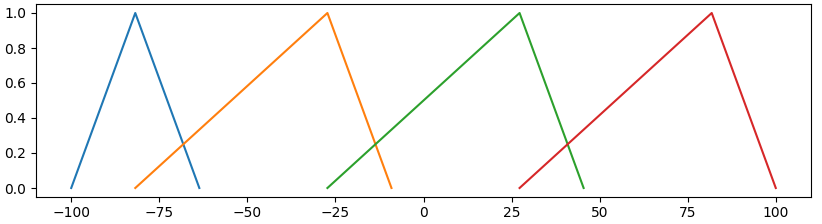
\includegraphics[scale=0.5]{images/mf_with_parameters.png}
	\caption{Ursprüngliche Fuzzy-Mengen}
	\label{mfs_urs}
\end{figure}

Die Anordnung ist gleich bei allen Mengen außer die Erste. Damit keine
Definitionslücken entstehen, verzichte ich auf die Trainierung der
beiden Grenzwertparametern. Neben dem Trainingsausschluß des ersten
Parameter der ersten Menge und des letzten der letzen Mengen, die die
Wertebereich bestimmen, werden auch weitere Einschränkungen angelegt.
Zum einen wird der Wert der Spitzenparameter (mittlerer Parameter) jeder
Funktion begrenzt, sodass er nicht kleiner als der linke Parameter, bzw.
größer als der rechte Parameter, wird. Der Spitzenparameter darf nicht gleich der linke oder rechte Parameter sein, weil es zur Undefiniertheit der Zugehörigkeitsfunktion führt.

Infolge des Austesten tauchten kritischen Fehler bezüglich der
Undefiniertheit der Zugehörigkeitsfunktionen auf. Diese Mangeln könnte
ich mit drei Einschränkungen aufheben. Die Beschränkungen fallen auf die
drei Parametern der Dreiecksfunktion.


\subsubsection{Zweiter Programmteil (Third Layer)}\label{zweiter-programmteil-third-layer}

Der zweite Programmteil enthält weniger Programmcode, aber dauert unter
Umständen länger. Die lange Laufzeit ergibt sich aus der Berechnung der
Permutationen der ZGF für alle Eingaben. Die Bibliothek
\(\textit{itertools}\) stellt mehrer Funktion bereit. Eine der Methoden
daraus berechnet das kartesische Produkt. Die Funktion kann mehrere
Mengen und einen \textbf{repeat}-Parameter entgegennehmen und liefert
eine Ergebnismenge. Die \textbf{repeat}-Variable gibt an, wie oft das
kartesische Produkt ausgeführt wird. Die Iteratorfunktion ist in der
Komplexitätsklasse \(TIME_{product()} \in O(n^k)\), mit \emph{n} gleich
die Anzahl der Elemente in der Angegebene Menge und \emph{k} gleich die
Anzahl der Ausführungen. Ein kleines Beispiel zur Verdeutlichung als
auch eine Implementierung des zweiten Programmteils wird unten gegeben.

\begin{lstlisting}[language=Python]
# itertools.product(l, r) builds the cartesian product of 
#the iterables (the list l).
# if r is equal to two, this would return the cartesian product 
#of the list l with itself (l x l).
# if r is three - (l x l x l). We use it here to get all 
#the combinations between the inputs
# Example: product((A, B), repeat=2) would result in the 
#list [(A, A), (A, B), (B, A), (B, B)]
for perm in it.product(range(self.num_sets), repeat=self.num_inputs):
	tmp = tf.ones(shape=(), dtype=tf.float64)
# loop from 0 to self.num_inputs and multiply the MF of an 
#input with index perm[i] with every other MF 
#with index from the permutation list
	for i in range(len(perm)):
		tmp = tf.multiply(premises[i][perm[i]], tmp)
	self.mf[index] = tmp
	index += 1
end = t.process_time()
\end{lstlisting}

Aus der Komplexitätsklasse ergibt sich, wie oft die äußere Schleife ausgeführt wird. Genauer gesagt, der Loop braucht so viele Iterationen bis zum Schluss wie die Gesamtzahl der Regeln. In der innere Schleife werden die Elemente in der Liste durchlaufen. Pro Iteration wird ein Element aus der Productliste betrachtet. Jeder Eintrag aus der Liste repräsentiert ein Index \textbf{perm{[}i{]}} einer Zugehörigkeitsfunktion für die entsprechende Eingabe \textbf{i}. Die Funktionen werden der Reihe nach mit einem Dummy-Tensor multiplizert. Auf dieser Weise werden die Prämisse jeder Regel definiert.

\subsection{Fourth Layer}\label{fourth-layer}

Im dritten Layer laut der Struktur des ANFIS-Models, werden alle Ergebnisse aus dem vorrigen Schicht normiert. Die Funktion besteht nur aus zwei Zeilen Code:
\begin{lstlisting}[language=Python]
def third_layer(self):
	# Reshape the MFs
	# Reshape the array, to be in the form of an array with 
	#num_rules items in it
	# sum the elements in the array along the 0th dimension
	self.mf_sum = tf.reduce_sum(tf.add(self.mf, [1e-10]), 0)
	# Normalize the MFs
	# Add all the items in the vector and divide every item in 
	#it with the sum of the elements
	# This way we get the normalized membership functions
	self.normalizedMFs = tf.divide(self.mf, self.mf_sum)
\end{lstlisting}

Mit der Funktion $\textbf{reduce\_sum()}$ werden die Einträge in einem Array, bzw. Matrix oder Vektor, zusammensumiert. Es kann einen zusätzlichen Parameter angegeben werden, der in der Dokumentation als $\textbf{axis}$ beschriftet ist und der angibt, welche Achse entlang die Elemente summiert werden sollen. Wie man am oberen Programmcode erkennt, werden hier die Elemente die 0. Achse entlang summiert. Wenn wir eine Matrix betrachten würden, heißt das für die Summe, dass die Elemente in einer Spalte summiert werden. Das Ergebnis der Summierung wird entsprechend in einer Variable abgespeichert, da wir einen zwei-Dimensionalen Array mit jeweils einen Eintrag in der zweite Dimension, erhalten wir eine Zahl. Schließlich werden alle Zugehörigkeitsfunktionen durch diesen Wert geteilt. Auf diesem Weg wird das Ergebnis der Prämissen normiert und ihre Summe gleich $\emph{1}$.

\subsection{Fifth Layer}\label{fifth-layer}

Die fünfte Schicht soll das Ergebnis aus jeder Konklusionsfunktion berechnen. Die Ausgabe erhalten wird, in dem die Eingangsgrößen in jeden Konklusionsfunktion eingesetzt werden und der Zutriffswert der Regeln an dem Funktionswert multipliziert werden. Durch die Normalisierung der Eintretungsgrößen erhalten wir eine Summe der Gewichte von 1, also ein Ergebnis mit Faktor kleiner 1 wird ausgegeben.

\begin{lstlisting}[language=Python]
def fifth_layer(self):
	# multiply every premis with its coresponding conclusion function
	# we get a vektor of results with each result having a factor less than 1
	self.outputs = tf.multiply(self.normalizedMFs, self.conclusions)
\end{lstlisting}

\subsection{Sixth Layer}\label{sixth-layer}

Die Summe aller Werten und das eigentliche Ergebnis für ein gegebenes Kandidat $\textbf{X}$ wird in der letzen (sechsten) Schicht berechnet. Dies erfolgt in einem Einzeiler:

\begin{lstlisting}[language=Python]
def sixth_layer(self):
	self.result = tf.reduce_sum(self.outputs, 0)
\end{lstlisting}

\section{Optimisierungsfunktion}\label{optimisierungsfunktion}

Nachdem das Neuronale Model aufgebaut wird, folgt die Definition des Optimierungsverfahren. In der Literatur, auch in der Praxis, wird die Kleinste-Quadrate Funktion verwendet. Auch hier habe ich diese eingesetzt. Als nächstes muss der Optimiser definiert werden. Die zwei bekanntesten sind $\emph{GradientDescentOptimizer}$ und $\emph{AdamOptimizer}$. Nach zahlreichem Testen der beidein Optimizer bin ich zu der überzeugung gekommen, dass der $\emph{AdamOptimizer}$ besser geeignet ist. Unten ist die Definition der Optimierungsfunktion gegeben.

\begin{lstlisting}[language=Python]
def optimize_method(self):
	self.loss = tf.losses.mean_squared_error(self.y, self.result)
	# self.loss = tf.losses.huber_loss(self.y, self.result)
	
	# self.optimizer =  
	#tf.train.GradientDescentOptimizer(learning_rate=0.01)
	#.minimize(self.loss)
	self.optimizer =
		 tf.train.AdamOptimizer(learning_rate=0.1).minimize(self.loss)
	# self.optimizer =
	# tf.train.RMSPropOptimizer(learning_rate=0.1).minimize(self.loss)
\end{lstlisting}
 
Wie üblich die Fehlerate ergibt sich aus dem Soll- und Istergebnis.
Weiterhin erhalten wir den Optimierer durch einen simplen Codeaufruf,
während dessen auch einen Lernrate gegeben wird. Normalerweise wird die
Lernrate mit einem Wert von 0.1 gesetzt.


\section{Trainingsfunktion}\label{trainingsfunktion}

Mit den oben erklärten Funktionen kann einen ANFIS-Model mit beliebigen
Eigenschaften erstellt werden. Nach dem Ausbau folgt das eigentliche
Lernen. Darum habe ich eine separate Methode definiert, die den Ablauf
beim Lernen beschreibt.
%\begin{lstlisting}
%	# PSEUDOCODE HERE
%	
%\end{lstlisting}

\begin{algorithm}
	\caption{Training function}
	\begin{algorithmic}[1]
		\REQUIRE initialize $statistic\_arrays$
		\STATE create $before\_training\_graphics$
		\IF{$gradient\_type\equal 0$}
			\STATE $train\_stocastic()$
		\ELSIF{$gradient\_type\equal 1$}
			\STATE $train\_mini\_batch()$
		\ELSE
			\STATE $train\_batch()$
		\ENDIF
		\STATE create $after\_training\_graphics$
		\STATE save data
	\end{algorithmic}
\end{algorithm}

Die Trainingsfunktion kann in vier Teile abgegrenzt werden. In dem ersten Teil fallen alle Operationen für die Aufzeichnung der Grafiken vor dem Lernen. Im zweiten Teil fällt der Lernzug. Danach kommt entsprechend die Zeichnung des 
geänderten Models. Zum Schluss werden alle Daten in Dateien abgespeichert.

Im nächsten Kapitel wird das beschriebene Programm getestet. Die Tests haben zum Ziel einen Verstand zu verschaffen, wie schell das Modell lernt und wie das Modell am besten konfiguriert werden kann.